\section{Cliente}
\subsection{Area Privata}
\emph{My Area} (Figura~\ref{fig:myarea-client}) mostra:
\begin{itemize}
    \item Elenco dei ristoranti preferiti
    \item Elenco delle recensioni scritte
\end{itemize}

\begin{figure}[H]
    \centering
    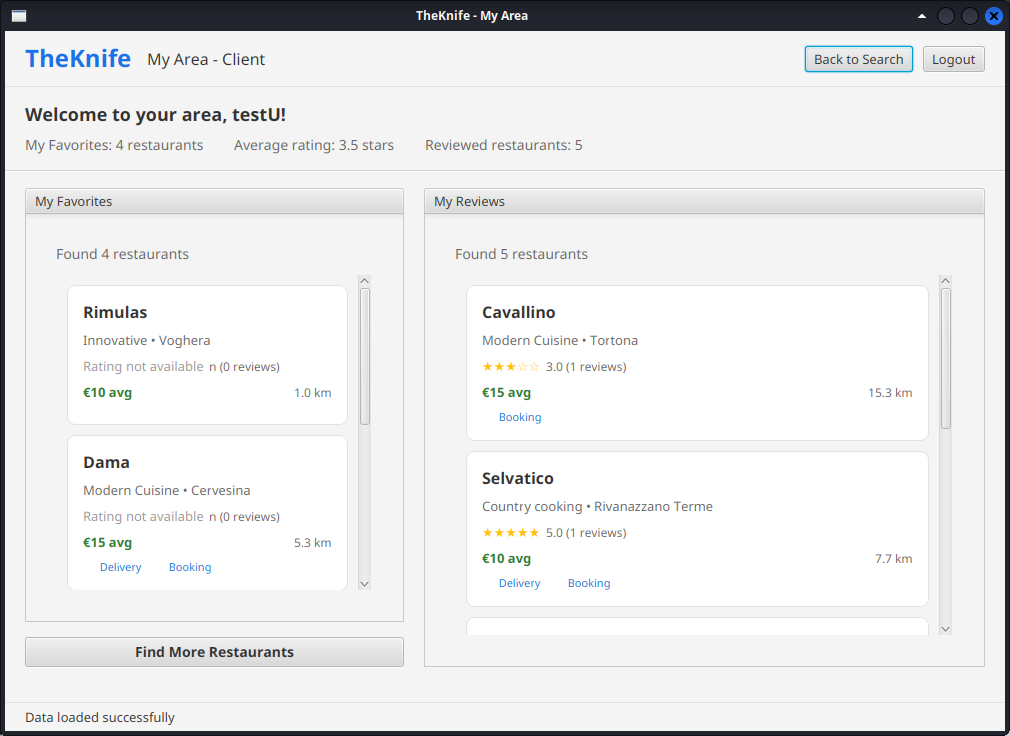
\includegraphics[width=0.8\textwidth]{images/myarea-client.png}
    \caption{Schermata Area Privata Cliente}
    \label{fig:myarea-client}
\end{figure}

\subsection{Recensioni}
Dalla vista del dettaglio del ristorante (Figura~\ref{fig:restaurant}), l'utente può
aggiungerlo ai preferiti con \emph{Add to Favourites} o scrivere una recensione.
Per scrivere una recensione, premere il pulsante 
\emph{Write a Review}, selezionare le stelle da 1 a 5 e inserire un commento.
Le recensioni possono essere modificate o cancellate in qualsiasi da \emph{My Area}.
\begin{figure}[H]
    \centering
    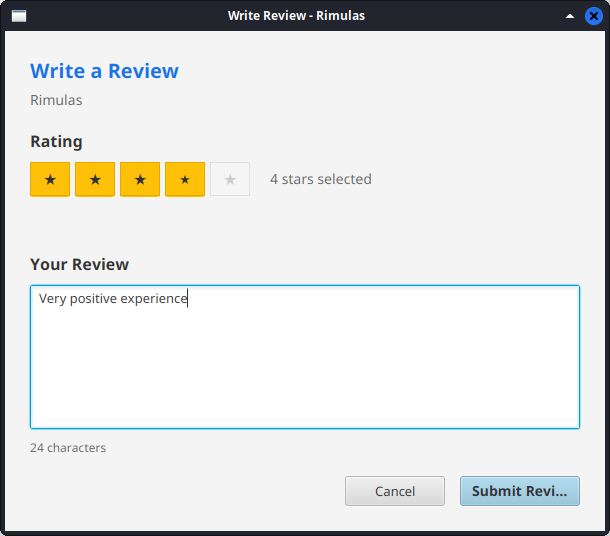
\includegraphics[width=0.8\textwidth]{images/review.png}
    \caption{Schermata di scrittura recensione}
    \label{fig:review}
\end{figure}